% ---
% Reemplaza líneas 3253–3394 de Docs/Technical_Report.tex.
% Decisiones que lo respaldan: D-006, D-009, D-022, H-002.
% Capítulo 4 desde el 2026-10-14 (antes §5).
% ---

\subsection{Análisis de imágenes DICOM}

\subsubsection{Dimensiones y características técnicas}

La Figura~\ref{fig:image_dimensions} muestra la
distribución de dimensiones de las mamografías
completas en la muestra analizada.

\begin{figure}[htbp]
  \centering
  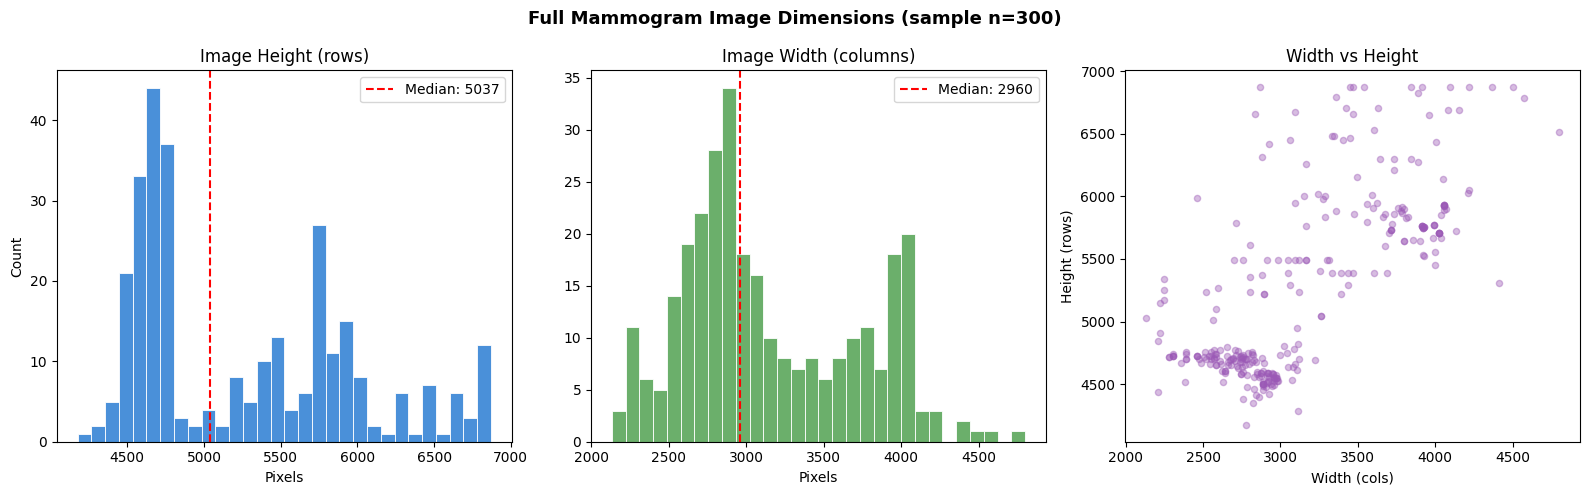
\includegraphics[width=0.8\textwidth]{Figures/D1_image_dimensions.png}
  \caption{Distribución de dimensiones (altura y anchura en píxeles) de las mamografías completas (muestra n\,=\,300).}
  \label{fig:image_dimensions}
\end{figure}

% fuente: D-009; 1_EDA.ipynb
Las mamografías completas presentan dimensiones
medianas de 5\,037\,$\times$\,2\,960 píxeles con
profundidad de 16 bits, lo que confirma que su tamaño
es incompatible con la entrada directa a un circuito
cuántico. Este hallazgo valida la decisión de diseño
de trabajar con recortes de la región de interés a
resolución original, de los que se extraen
características radiómicas (capítulo~\ref{sec:metodologia},
sección~\ref{sec:modulo3}) en lugar de las mamografías completas.

% fuente: H-002; 1_metadatos_dicom.csv
La inspección de los metadatos DICOM reveló que las
imágenes del dataset son de tipo \textit{Secondary
Capture} (\texttt{SOPClassUID}:
1.2.840.10008.5.1.4.1.1.7), generadas mediante
MATLAB (\texttt{SecondaryCapture}\allowbreak\texttt{DeviceManufacturer}:
MathWorks) como parte del proceso de digitalización
y curaduría del CBIS-DDSM. La convención fotométrica
es \texttt{MONOCHROME2} de forma uniforme en todo el
dataset, lo que elimina la necesidad de inversión de
píxeles en el preprocesamiento.

\subsubsection{Variabilidad inter-escáner}

% fuente: H-002; 1_metadatos_dicom.csv
Ninguna de las 3\,103 mamografías distintas incluye las etiquetas
\texttt{Manufacturer}, \texttt{PixelSpacing} ni
\texttt{ImagerPixelSpacing}; las tres faltan en los archivos
DICOM (véase la Figura~\ref{fig:manufacturers} del Anexo~\ref{anx:figuras_eda}).
Como consecuencia, no es posible un análisis de
variabilidad entre escáneres a partir de metadatos, y las
características de forma quedan en píxeles sin escala física;
como el DDSM original se digitalizó con escáneres de distinta
resolución, el mismo tamaño físico da distinto número de
píxeles según el digitalizador, lo que se declara como
limitación. Todas las imágenes corresponden a la modalidad MG,
con profundidad de 16 bits y convención fotométrica
\texttt{MONOCHROME2}.

\subsubsection{Distribución de intensidades de píxeles}

La comparación cuantitativa de las distribuciones estadísticas
de intensidad de píxeles (media, desviación estándar y máximo)
entre casos benignos y malignos en las imágenes de ROI se presenta
en la Figura~\ref{fig:pixel_intensities} del Anexo~\ref{anx:figuras_eda}.

% fuente: D-006, D-022; 1_EDA.ipynb
Las imágenes recortadas presentan valores de
intensidad media en el rango de 45\,000--50\,000
sobre un máximo posible de 65\,535 (16 bits),
con máximos frecuentemente en el límite superior.
Las distribuciones de casos benignos y malignos
muestran solapamiento considerable en las tres
estadísticas analizadas, confirmando que la
información discriminativa no reside en estadísticas
globales de intensidad sino en patrones texturales
y morfológicos de orden superior, que son precisamente
los que capturan las \textit{features} radiómicas
de PyRadiomics.

\subsubsection{Galería de casos representativos}

Una galería visual de casos representativos que ilustra la
mamografía completa, la máscara binaria ROI y la imagen recortada
de la lesión se exhibe en la Figura~\ref{fig:sample_gallery} del
Anexo~\ref{anx:figuras_eda}.

La galería ilustra visualmente las diferencias
morfológicas descritas en el análisis de variables
clínicas: las masas malignas muestran bordes
irregulares y espiculados, mientras que las masas
benignas presentan contornos lisos y bien definidos.
En las calcificaciones, la distinción visual entre
clases es menos evidente, consistente con el hallazgo
de que PLEOMORPHIC es el tipo morfológico más
frecuente en ambas clases.

La Figura~\ref{fig:roi_overlays} muestra la
superposición de la máscara ROI sobre la mamografía
completa para cuatro casos seleccionados.

\begin{figure}[htbp]
  \centering
  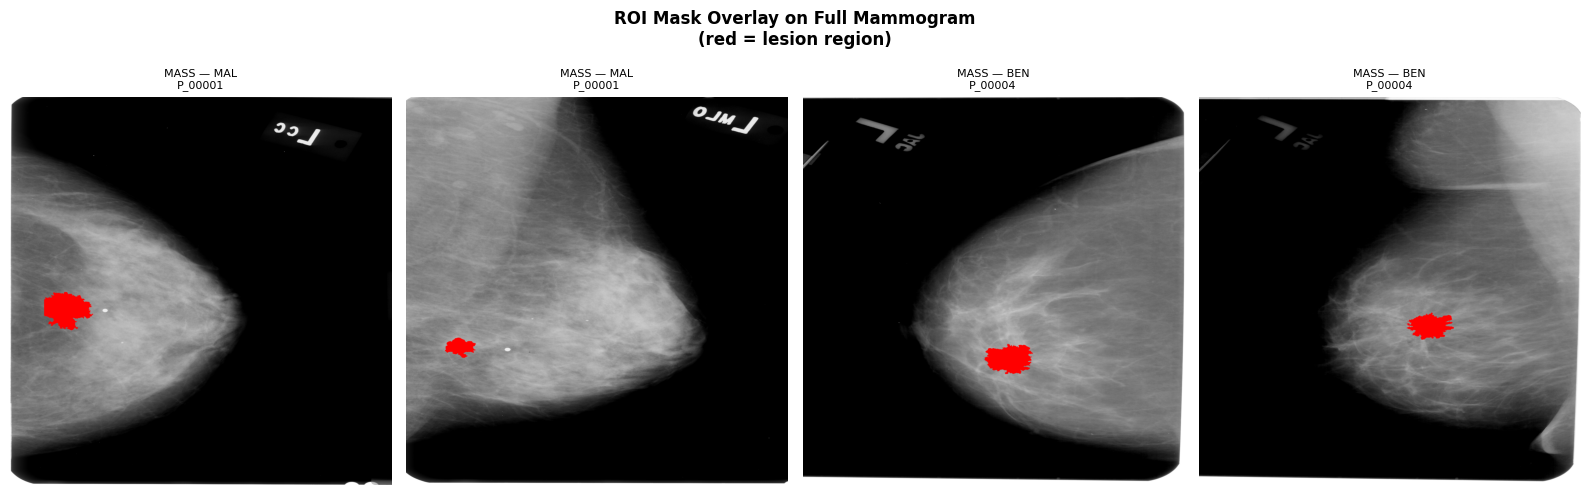
\includegraphics[width=\textwidth]{Figures/D5_roi_overlays.png}
  \caption{Superposición de la máscara ROI (región en rojo) sobre la mamografía completa para cuatro casos representativos.}
  \label{fig:roi_overlays}
\end{figure}

La visualización muestra que las máscaras ROI
delimitan la región de la lesión dentro de la
mamografía completa, lo que respalda su uso como
guía para el recorte. La verificación sistemática
del preprocesamiento encontró 80 máscaras con
dimensiones distintas a las de su mamografía, que
se tratan en la sección~\ref{sec:modulo2}.
